%%%%%%%%%%%%%%%%%%%%%%%%%%%%%%%%%%%%%%%%%%%%%%%%%%%%%%%%%%%%%%%%%%%%%%%%%%%%%%%%%%%%%%%%%%%%%%%%
%
% CS484 Written Question Template
%
% Acknowledgements:
% The original code is written by Prof. James Tompkin (james_tompkin@brown.edu).
% The second version is revised by Prof. Min H. Kim (minhkim@kaist.ac.kr).
%
% This is a LaTeX document. LaTeX is a markup language for producing 
% documents. Your task is to fill out this document, then to compile 
% it into a PDF document. 
%
% 
% TO COMPILE:
% > pdflatex thisfile.tex
%
% If you do not have LaTeX and need a LaTeX distribution:
% - Personal laptops (all common OS): www.latex-project.org/get/
% - We recommend latex compiler miktex (https://miktex.org/) for windows,
%   macTex (http://www.tug.org/mactex/) for macOS users.
%   And TeXstudio(http://www.texstudio.org/) for latex editor.
%   You should install both compiler and editor for editing latex.
%   The another option is Overleaf (https://www.overleaf.com/) which is 
%   an online latex editor.
%
% If you need help with LaTeX, please come to office hours. 
% Or, there is plenty of help online:
% https://en.wikibooks.org/wiki/LaTeX
%
% Good luck!
% Min and the CS484 staff
%
%%%%%%%%%%%%%%%%%%%%%%%%%%%%%%%%%%%%%%%%%%%%%%%%%%%%%%%%%%%%%%%%%%%%%%%%%%%%%%%%%%%%%%%%%%%%%%%%
%
% How to include two graphics on the same line:
% 
% \includegraphics[\width=0.49\linewidth]{yourgraphic1.png}
% \includegraphics[\width=0.49\linewidth]{yourgraphic2.png}
%
% How to include equations:
%
% \begin{equation}
% y = mx+c
% \end{equation}
% 
%%%%%%%%%%%%%%%%%%%%%%%%%%%%%%%%%%%%%%%%%%%%%%%%%%%%%%%%%%%%%%%%%%%%%%%%%%%%%%%%%%%%%%%%%%%%%%%%

\documentclass[11pt]{article}

\usepackage[english]{babel}
\usepackage[utf8]{inputenc}
\usepackage[colorlinks = true,
            linkcolor = blue,
            urlcolor  = blue]{hyperref}
\usepackage[a4paper,margin=1.5in]{geometry}
\usepackage{stackengine,graphicx}
\usepackage{fancyhdr}
\setlength{\headheight}{15pt}
\usepackage{microtype}
\usepackage{times}
\usepackage{booktabs}
\usepackage{listings}
\usepackage{xcolor}
\lstdefinestyle{codestyle}{
	frame=single,
	basicstyle=\ttfamily\footnotesize,
	keywordstyle=\bfseries\color{magenta},
	commentstyle=\itshape\color{gray},
	stringstyle=\color{orange},
	numberstyle=\sffamily\scriptsize\color{gray},
	showspaces=false,
	showstringspaces=false,
	showtabs=false,
	tabsize=4,
	breakatwhitespace=false,
	breaklines=true,
	keepspaces=true,
	captionpos=b,
	numbers=left,
	numbersep=5pt}
\lstset{style=codestyle}

\frenchspacing
\setlength{\parindent}{0cm} % Default is 15pt.
\setlength{\parskip}{0.3cm plus1mm minus1mm}

\pagestyle{fancy}
\fancyhf{}
\lhead{Homework Writeup}
\rhead{CS484}
\rfoot{\thepage}

\date{}

\title{\vspace{-1cm}Homework 5 Writeup}


\begin{document}
\maketitle
\vspace{-3cm}
\thispagestyle{fancy}

\section*{Code Implementation and Details}
\subsection*{Feature Extraction}
\begin{lstlisting}[language=python]
def feature_extraction(img, feature):
    """
    This function computes defined feature (HoG, SIFT) descriptors of the target image.

    :param img: a height x width x channels matrix,
    :param feature: name of image feature representation.

    :return: a number of grid points x feature_size matrix.
    """

    if feature == 'HoG':
        # HoG parameters
        win_size = (32, 32)
        block_size = (32, 32)
        block_stride = (16, 16)
        cell_size = (16, 16)
        nbins = 9
        deriv_aperture = 1
        win_sigma = 4
        histogram_norm_type = 0
        l2_hys_threshold = 2.0000000000000001e-01
        gamma_correction = 0
        nlevels = 64
        
        hog = cv2.HOGDescriptor(win_size, block_size, block_stride, cell_size, nbins, deriv_aperture, win_sigma, histogram_norm_type, l2_hys_threshold, gamma_correction, nlevels)
        hog_features = hog.compute(img)
        
        return hog_features.reshape(-1, 36)
    elif feature == 'SIFT':
        sift = cv2.SIFT_create()
        step_size = 20
        keypoints = [cv2.KeyPoint(x, y, step_size) for y in range(0, img.shape[0], step_size) for x in range(0, img.shape[1], step_size)]
        keypoints, descriptors = sift.compute(img, keypoints)
        
        
        if descriptors is None:
            return np.zeros((0, 128), dtype=np.float32)
        return descriptors
\end{lstlisting}

\begin{itemize}
    \item \textbf{HoG Descriptor} For HoG Descriptor, I simply used cv2.HoGDescriptor function to obtain HoG feature points. Then I reshaped the output into -1*36 size, which automatically makes the row number.
    \item \textbf{SIFT Descriptor} For SIFT Descriptor, I implemented the regular grid feature extraction with grid size 20. First I devided the image into 20*20 size grids, and for each grid made keypoints with cv2.Keypoint function. Then for each keypoints I computed the SIFT descriptor. If there are no descriptors found, the code gives zero array for output.
\end{itemize}
\subsection*{Principal Component Analysis}
\begin{lstlisting}[language=python]
def get_features_from_pca(feat_num, feature):

    vocab = np.load(f'vocab_{feature}.npy')
    
    vocab_mean = np.mean(vocab, axis=0)
    vocab_centered = vocab - vocab_mean

    covariance_matrix = np.cov(vocab_centered, rowvar=False)

    eigen_values, eigen_vectors = np.linalg.eigh(covariance_matrix)

    idx = np.argsort(eigen_values)[::-1]
    principal_components = eigen_vectors[:, idx[:feat_num]]

    reduced_vocab = np.dot(vocab_centered, principal_components)

    return reduced_vocab
\end{lstlisting}
\begin{itemize}
    \item First, from the loaded vocabulary I centered it by extracting the mean.
    \item Then, with the centered vocabulary I calculated the covariance matrix, and performed eigenvalue decompostition to obtain eigenvalues and vectors.
    \item I sorted the eigenvalues from largest one to the smallest one, and then chose the eigenvectors corresponding to largest feat\_num indices. 
    \item Finally, I obtained the reduced vocabulary by making a dot product with the centered vocabulary and selected eigenvectors.
\end{itemize}
\subsection*{Bag of Words}
\begin{lstlisting}[language=python]
def get_bags_of_words(image_paths, feature):
    vocab = np.load(f'vocab_{feature}.npy')

    vocab_size = vocab.shape[0]

    bags_of_words = np.zeros((len(image_paths), vocab_size))

    for i, path in enumerate(image_paths):
        img = cv2.imread(path)
        features = feature_extraction(img, feature)

        distances = pdist(features, vocab)
        closest_vocab = np.argmin(distances, axis=1)

        for idx in closest_vocab:
            bags_of_words[i, idx] += 1

        bags_of_words[i, :] /= linalg.norm(bags_of_words[i, :])

    return bags_of_words
\end{lstlisting}
\begin{itemize}
    \item First I made an empty array with size of the number of test images and vocabulary size, to use it as histogram.
    \item For each test images, I extracted the feature points with pre-implemented feature\_extraction function.
    \item Calculated the distance between the feature vectors of the test image and the vocabulary by pdist function.
    \item Then I sorted the distances array to get the vocabulary that is closest to the given image's feature vectors.
    \item If a typical vocabulary is chosen as the closest one, then I incremented the count of the histogram for that index of vocabulary.
    \item Finally, I applied L2 normalization for the histogram, by deviding the feature vector with the size of the vector.
\end{itemize}
\subsection*{Spatial Pyramid Representation}
\begin{lstlisting}[language=python]
def get_spatial_pyramid_feats(image_paths, max_level, feature):

    vocab = np.load(f'vocab_{feature}.npy')
    vocab_size = vocab.shape[0]

    d = 0
    for l in range(max_level + 1):
        d += (vocab_size * (4 ** l))
    pyramid_features = np.zeros((len(image_paths), d))

    for i, path in enumerate(image_paths):
        img = cv2.imread(path)
        h, w = img.shape[:2]
        current_feature = []
        for l in range(max_level + 1):
            sub_h, sub_w = h // (2 ** l), w // (2 ** l)
            for y in range(2 ** l):
                for x in range(2 ** l):
                    sub_img = img[y*sub_h:(y+1)*sub_h, x*sub_w:(x+1)*sub_w]
                    sub_features = feature_extraction(sub_img, feature)

                    distances = pdist(sub_features, vocab)
                    closest_vocab_indices = np.argmin(distances, axis=1)

                    hist = np.zeros(vocab_size)
                    for idx in closest_vocab_indices:
                        hist[idx] += 1

                    weight = 2 ** (-max_level+l-1) if l > 0 else -max_level
                    current_feature.extend(weight * hist)

        normalized_feature = np.array(current_feature) / linalg.norm(current_feature)

        pyramid_features[i, :len(normalized_feature)] = normalized_feature

    return pyramid_features    
\end{lstlisting}
\begin{itemize}
    \item First, I initialized the feature map with the size of number of test images, and the total number of subimages, which is $4^l*vocab\_size$ for each level of pyramid.
    \item Iterate through the test images and the level of spatial pyramid. For each level, the images are divided into $4^l$ subimages.
    \item For each subimages, feature vectors are extracted, and the closest vocabulary is calculated, simillar to the bag of words. 
    \item After computing the histogram, weight for spational imformation is multplied to the histogram.
    \item Finally, the histogram is L2 normalized, and applied to the total pyramid feature array.
\end{itemize}
\subsection*{Multi-Class SVM}
\begin{lstlisting}[language=python]
def svm_classify(train_image_feats, train_labels, test_image_feats, kernel_type):

    categories = np.unique(train_labels)

    n_categories = len(categories)

    svms = {category: svm.SVC(kernel=kernel_type.lower(), C=10) for category in categories}

    for category in categories:
        labels = (train_labels == category).astype(int)
        svms[category].fit(train_image_feats, labels)

    predictions = np.zeros((len(test_image_feats), n_categories))
    for i, category in enumerate(categories):
        predictions[:, i] = svms[category].decision_function(test_image_feats)

    predicted_categories = categories[np.argmax(predictions, axis=1)]

    return predicted_categories    
\end{lstlisting}
\begin{itemize}
    \item Number of categories to be classified is determined by extracting the unique categories from train labels.
    \item Using svm.SVC function, I made the svm object with the given kernel and lambda value for each categories. Since lambda value is the hyperparamter, I tired some different values, which will be explained later.
    \item For each of categories, I made binary label which gives positive label for the labels in the target category, and negative label for the labels not in it.
    \item Then, I trained the SVM model for each of categories by fitting the train image features to the train lables. This gives 15 trained SVM model for each of 15 categories.
    \item Test image features are used as input in the model, and the prediction probability for each classes are calcuated by SVM decision function for each class.
\end{itemize}
\section*{Analysis of the result}
\subsection*{HoG Descriptor VS SIFT Descriptor}
\begin{table*}[h]
    \centering
    \begin{tabular}{lr}
        \toprule
        Descriptor & Accuracy (percent) \\
        \midrule
        HoG & 59.3 \\
        SIFT & 60.9 \\
        \bottomrule
    \end{tabular}
    \caption{Accuracy Comparison between HoG and SIFT Descriptor}
\end{table*}
Accuracy was compared between HoG and SIFT Descriptor. Bag of Words representation was used, and fixed linear kernel for SVM with lambda=10.
SIFT Descriptor showed higher accuracy for about 1.6 percent.

\subsection*{PCA Visualization of the Vocabulary}

\begin{figure}[h]
    \centering
    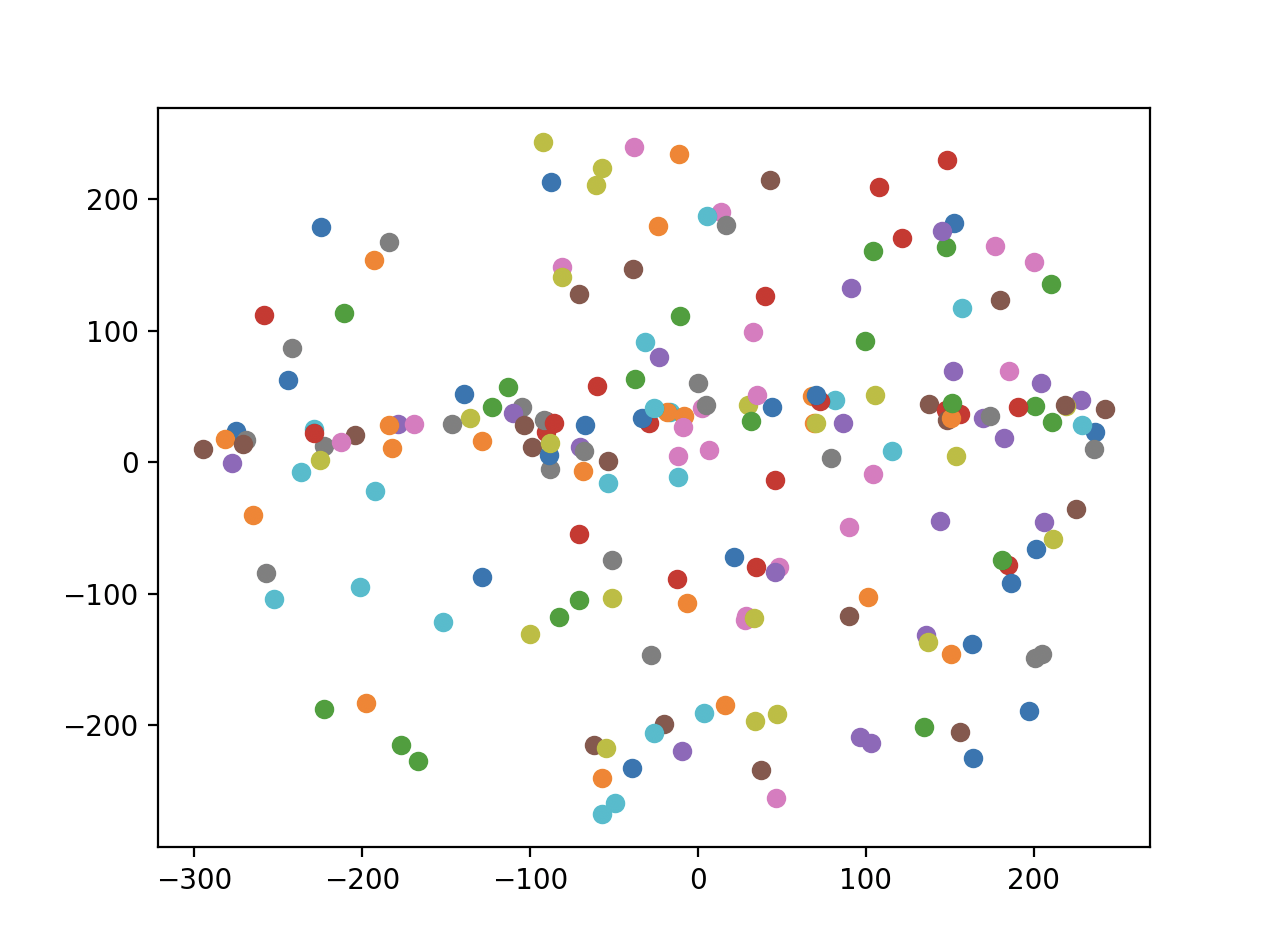
\includegraphics[width=6cm]{../pca_dimension2.png}
    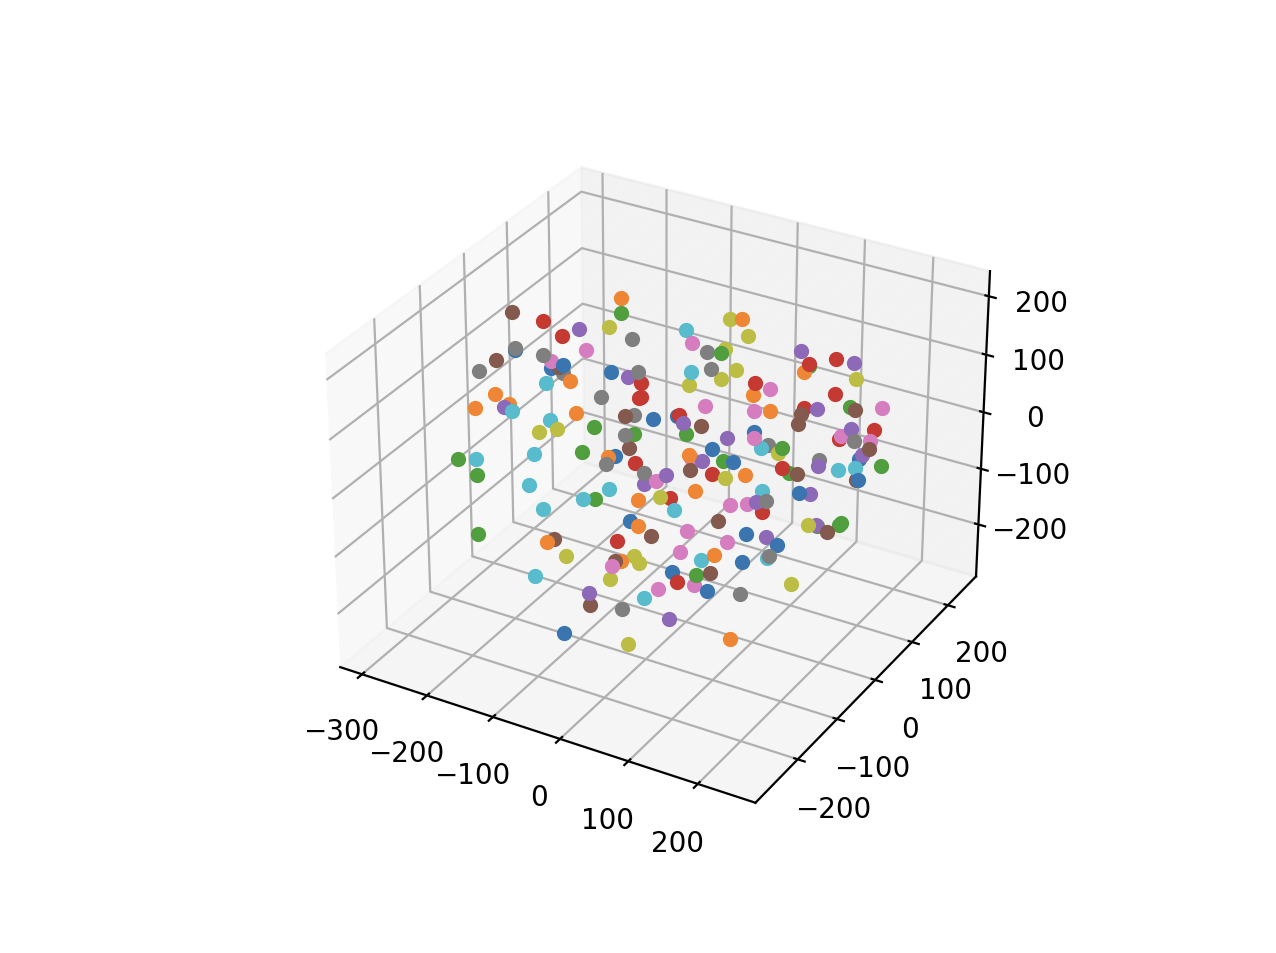
\includegraphics[width=6cm]{../pca_dimension3.png}
    \caption{\emph{Left:} Reduction to dimension 2 \emph{Right:} Reduction to dimension 3}
    \label{fig:result1}
\end{figure}
This is the result of PCA for vocabulary. SIFT descriptor was used to extract features. Left figure is reduction to dimension 2, and right figure is reduction to dimension 3.

\subsection*{Linear Kernel VS RBF Kernel}
\begin{table*}[h]
    \centering
    \begin{tabular}{lr}
        \toprule
        Kernel Type & Accuracy (percent) \\
        \midrule
        Linear & 60.9 \\
        RBF & 63.5 \\
        \bottomrule
    \end{tabular}
    \caption{Accuracy Comparison between Linear and RBF kernel}
\end{table*}
The train features were extracted with SIFT, and represented with bag of word without spatial pyramid. Bag of words representation was used without spatial pyramid. Usage of RBF kernel showed about 2.6 percent improvement in accuracy. 
\subsection*{Effect of Spatial Pyramid Representation}
\begin{table*}[h]
    \centering
    \begin{tabular}{lr}
        \toprule
        Representation & Accuracy (percent) \\
        \midrule
        Bag of Words & 63.5 \\
        Bag of Words + Spatial Pyramid & 64.0 \\
        \bottomrule
    \end{tabular}
    \caption{The effect of spatial pyramid representation on accuracy}
\end{table*}
Adding spatial pyramid representation on bag of words improved accuracy about 0.5 percent. SIFT descriptor was used for feature extraction, and RBF kernel was used.
\subsection*{Choosing Hyperparamter}
Hyperparamter in this project is the lambda value of multi-class SVM. Lambda, which is written as ``C'' in svm function, decides the intensity of normalization in model. When C is large, the model tries to fit more on data, and when C is small, the model tries to find more generalized solution. Decision of C is important since too large or too small C could bring overfitting of underfitting. 

I varied the value of C from 0.1 to 100 with other parameters fixed, since C could be found by log scaling. I chosed the C value which showed the highest accuracy.

\begin{table*}[h]
    \centering
    \begin{tabular}{lr}
        \toprule
        C & Accuracy (percent) \\
        \midrule
        0.1 & 57.3 \\
        1 & 63.5 \\
        10 & 64.0 \\
        100 & 62.9 \\
        \bottomrule
    \end{tabular}
    \caption{The effect of spatial pyramid representation on accuracy}
\end{table*}
I used SIFT descriptor for feature extraction, and RBF kernel. Bag of words representation was used without spatial pyramid.
Since the accuracy was highest when C=10, I choosed C for 10.
\end{document}